% Options for packages loaded elsewhere
\PassOptionsToPackage{unicode}{hyperref}
\PassOptionsToPackage{hyphens}{url}
\PassOptionsToPackage{dvipsnames,svgnames,x11names}{xcolor}
%
\documentclass[
  ,doc,11pt, twoside,floatsintext]{apa6}
\usepackage{amsmath,amssymb}
\usepackage{lmodern}
\usepackage{iftex}
\ifPDFTeX
  \usepackage[T1]{fontenc}
  \usepackage[utf8]{inputenc}
  \usepackage{textcomp} % provide euro and other symbols
\else % if luatex or xetex
  \usepackage{unicode-math}
  \defaultfontfeatures{Scale=MatchLowercase}
  \defaultfontfeatures[\rmfamily]{Ligatures=TeX,Scale=1}
\fi
% Use upquote if available, for straight quotes in verbatim environments
\IfFileExists{upquote.sty}{\usepackage{upquote}}{}
\IfFileExists{microtype.sty}{% use microtype if available
  \usepackage[]{microtype}
  \UseMicrotypeSet[protrusion]{basicmath} % disable protrusion for tt fonts
}{}
\makeatletter
\@ifundefined{KOMAClassName}{% if non-KOMA class
  \IfFileExists{parskip.sty}{%
    \usepackage{parskip}
  }{% else
    \setlength{\parindent}{0pt}
    \setlength{\parskip}{6pt plus 2pt minus 1pt}}
}{% if KOMA class
  \KOMAoptions{parskip=half}}
\makeatother
\usepackage{xcolor}
\usepackage{graphicx}
\makeatletter
\def\maxwidth{\ifdim\Gin@nat@width>\linewidth\linewidth\else\Gin@nat@width\fi}
\def\maxheight{\ifdim\Gin@nat@height>\textheight\textheight\else\Gin@nat@height\fi}
\makeatother
% Scale images if necessary, so that they will not overflow the page
% margins by default, and it is still possible to overwrite the defaults
% using explicit options in \includegraphics[width, height, ...]{}
\setkeys{Gin}{width=\maxwidth,height=\maxheight,keepaspectratio}
% Set default figure placement to htbp
\makeatletter
\def\fps@figure{htbp}
\makeatother
\setlength{\emergencystretch}{3em} % prevent overfull lines
\providecommand{\tightlist}{%
  \setlength{\itemsep}{0pt}\setlength{\parskip}{0pt}}
\setcounter{secnumdepth}{-\maxdimen} % remove section numbering
% Make \paragraph and \subparagraph free-standing
\ifx\paragraph\undefined\else
  \let\oldparagraph\paragraph
  \renewcommand{\paragraph}[1]{\oldparagraph{#1}\mbox{}}
\fi
\ifx\subparagraph\undefined\else
  \let\oldsubparagraph\subparagraph
  \renewcommand{\subparagraph}[1]{\oldsubparagraph{#1}\mbox{}}
\fi
\newlength{\cslhangindent}
\setlength{\cslhangindent}{1.5em}
\newlength{\csllabelwidth}
\setlength{\csllabelwidth}{3em}
\newlength{\cslentryspacingunit} % times entry-spacing
\setlength{\cslentryspacingunit}{\parskip}
\newenvironment{CSLReferences}[2] % #1 hanging-ident, #2 entry spacing
 {% don't indent paragraphs
  \setlength{\parindent}{0pt}
  % turn on hanging indent if param 1 is 1
  \ifodd #1
  \let\oldpar\par
  \def\par{\hangindent=\cslhangindent\oldpar}
  \fi
  % set entry spacing
  \setlength{\parskip}{#2\cslentryspacingunit}
 }%
 {}
\usepackage{calc}
\newcommand{\CSLBlock}[1]{#1\hfill\break}
\newcommand{\CSLLeftMargin}[1]{\parbox[t]{\csllabelwidth}{#1}}
\newcommand{\CSLRightInline}[1]{\parbox[t]{\linewidth - \csllabelwidth}{#1}\break}
\newcommand{\CSLIndent}[1]{\hspace{\cslhangindent}#1}
\ifLuaTeX
\usepackage[bidi=basic]{babel}
\else
\usepackage[bidi=default]{babel}
\fi
\babelprovide[main,import]{english}
% get rid of language-specific shorthands (see #6817):
\let\LanguageShortHands\languageshorthands
\def\languageshorthands#1{}
% Manuscript styling
\usepackage{upgreek}
\captionsetup{font=singlespacing,justification=justified}

% Table formatting
\usepackage{longtable}
\usepackage{lscape}
% \usepackage[counterclockwise]{rotating}   % Landscape page setup for large tables
\usepackage{multirow}		% Table styling
\usepackage{tabularx}		% Control Column width
\usepackage[flushleft]{threeparttable}	% Allows for three part tables with a specified notes section
\usepackage{threeparttablex}            % Lets threeparttable work with longtable

% Create new environments so endfloat can handle them
% \newenvironment{ltable}
%   {\begin{landscape}\begin{center}\begin{threeparttable}}
%   {\end{threeparttable}\end{center}\end{landscape}}
\newenvironment{lltable}{\begin{landscape}\begin{center}\begin{ThreePartTable}}{\end{ThreePartTable}\end{center}\end{landscape}}

% Enables adjusting longtable caption width to table width
% Solution found at http://golatex.de/longtable-mit-caption-so-breit-wie-die-tabelle-t15767.html
\makeatletter
\newcommand\LastLTentrywidth{1em}
\newlength\longtablewidth
\setlength{\longtablewidth}{1in}
\newcommand{\getlongtablewidth}{\begingroup \ifcsname LT@\roman{LT@tables}\endcsname \global\longtablewidth=0pt \renewcommand{\LT@entry}[2]{\global\advance\longtablewidth by ##2\relax\gdef\LastLTentrywidth{##2}}\@nameuse{LT@\roman{LT@tables}} \fi \endgroup}

% \setlength{\parindent}{0.5in}
% \setlength{\parskip}{0pt plus 0pt minus 0pt}

% Overwrite redefinition of paragraph and subparagraph by the default LaTeX template
% See https://github.com/crsh/papaja/issues/292
\makeatletter
\renewcommand{\paragraph}{\@startsection{paragraph}{4}{\parindent}%
  {0\baselineskip \@plus 0.2ex \@minus 0.2ex}%
  {-1em}%
  {\normalfont\normalsize\bfseries\itshape\typesectitle}}

\renewcommand{\subparagraph}[1]{\@startsection{subparagraph}{5}{1em}%
  {0\baselineskip \@plus 0.2ex \@minus 0.2ex}%
  {-\z@\relax}%
  {\normalfont\normalsize\itshape\hspace{\parindent}{#1}\textit{\addperi}}{\relax}}
\makeatother

% \usepackage{etoolbox}
\makeatletter
\patchcmd{\HyOrg@maketitle}
  {\section{\normalfont\normalsize\abstractname}}
  {\section*{\normalfont\normalsize\abstractname}}
  {}{\typeout{Failed to patch abstract.}}
\patchcmd{\HyOrg@maketitle}
  {\section{\protect\normalfont{\@title}}}
  {\section*{\protect\normalfont{\@title}}}
  {}{\typeout{Failed to patch title.}}
\makeatother

\usepackage{xpatch}
\makeatletter
\xapptocmd\appendix
  {\xapptocmd\section
    {\addcontentsline{toc}{section}{\appendixname\ifoneappendix\else~\theappendix\fi\\: #1}}
    {}{\InnerPatchFailed}%
  }
{}{\PatchFailed}
\usepackage{csquotes}
\setcounter{tocdepth}{3}
\setlength{\parskip}{5pt}
\linespread{1.5}
\usepackage{setspace}
\usepackage{tabu}
\usepackage{ragged2e}
\usepackage{graphicx}
\usepackage{hyperref}
\hypersetup{colorlinks = true, urlcolor = blue, linkcolor = blue, citecolor = red}
\shorttitle{}
\fancyheadoffset[L]{0pt}
\fancyhf{}
\fancyhead[RO,LE]{\small\thepage}
\renewcommand{\headrulewidth}{0pt}
\interfootnotelinepenalty=10000
\ifLuaTeX
  \usepackage{selnolig}  % disable illegal ligatures
\fi
\IfFileExists{bookmark.sty}{\usepackage{bookmark}}{\usepackage{hyperref}}
\IfFileExists{xurl.sty}{\usepackage{xurl}}{} % add URL line breaks if available
\urlstyle{same} % disable monospaced font for URLs
\hypersetup{
  pdftitle={Cross-cultural adaptation and psychometric studies of the Dysfunctional Beliefs and Attitudes about Sleep scale and the Sleep Problem Acceptance Questionnaire},
  pdflang={en-EN},
  colorlinks=true,
  linkcolor={Maroon},
  filecolor={Maroon},
  citecolor={Blue},
  urlcolor={blue},
  pdfcreator={LaTeX via pandoc}}

\title{Cross-cultural adaptation and psychometric studies of the Dysfunctional Beliefs and Attitudes about Sleep scale and the Sleep Problem Acceptance Questionnaire}
\author{\textsuperscript{}}
\date{}


\shorttitle{Subliminal Header}

\affiliation{\vspace{0.5cm}\textsuperscript{} }

\begin{document}
\maketitle

\clearpage

\mbox{}\thispagestyle{empty}\clearpage

\setcounter{page}{1}

\thispagestyle{empty}
\begin{center}
\vspace*{10mm}
\textbf{\Large Cross-cultural adaptation and psychometric studies of the DBAS-16 and SPAQ}\\

\begin{figure}[h]
\begin{center}

\includegraphics[width=!,totalheight=!,scale=0.18]{usp-brazao.jpg}
\end{center}
\end{figure}
{\setstretch{1.7} 
Projeto de qualificação\\
para\\ 
Obtenção do título de mestre em ciências\\
da Faculdade de Medicina\\
da Universidade de São Paulo  \\
Área de concentração: Psiquiatria  \\
apresentado por  \\ 
\smallskip
\textbf{Marwin M I B Carmo}\\
\smallskip
Orientação:  \\
Dra. Renatha El Rafihi Ferreira  \\
\smallskip
São Paulo, Outubro de 2022\\
}
\end{center}

\clearpage

\mbox{}\thispagestyle{empty}\clearpage

\textbf{Acknowledgment}

\bigskip

Lorem ipsum dolor sit amet, consetetur sadipscing elitr, sed diam nonumy eirmod tempor invidunt ut labore et dolore magna aliquyam erat, sed diam voluptua. At vero eos et accusam et justo duo dolores et ea rebum. Stet clita kasd gubergren, no sea takimata sanctus est Lorem ipsum dolor sit amet. Lorem ipsum dolor sit amet, consetetur sadipscing elitr, sed diam nonumy eirmod tempor invidunt ut labore et dolore magna aliquyam erat, sed diam voluptua. At vero eos et accusam et justo duo dolores et ea rebum. Stet clita kasd gubergren, no sea takimata sanctus est Lorem ipsum dolor sit amet. Lorem ipsum dolor sit amet, consetetur sadipscing elitr, sed diam nonumy eirmod tempor danke frederik invidunt ut labore et dolore magna aliquyam erat, sed diam voluptua. At vero eos et accusam et justo duo dolores et ea rebum. Stet clita kasd gubergren, no sea takimata sanctus est Lorem ipsum dolor sit amet.

\clearpage

\mbox{}\thispagestyle{empty}\clearpage

\begin{flushleft}
{\setstretch{1.0}
\tableofcontents
}
\end{flushleft}

\newpage

\clearpage

\mbox{}\thispagestyle{empty}\clearpage

\thispagestyle{empty}

\hypertarget{summary}{%
\section{Summary}\label{summary}}

Insomnia disorder is characterized by frequent complaints about the quality and quantity of sleep and may cause physical and psychological damage. Maladaptive beliefs about sleep were identified as reinforcers of insomnia. A insônia se caracteriza por queixas frequentes sobre a qualidade e quantidade de sono e tende a implicar em danos físicos e psicológicos à saúde do indivíduo. Crenças desadaptativas sobre o sono vem sendo identificados como fatores reforçadores da insônia e, com isto, tratamentos com foco nos aspectos cognitivos como a Terapia Cognitivo-Comportamental e a Terapia de Aceitação e Compromisso tem sido adotados por pesquisadores e clínicos, demonstrando efetividade. Como forma de avaliar essas cognições foram desenvolvidas escalas como a Dysfunctional Beliefs and Attitudes about Sleep Scale (DBAS-16), avaliando a força de concordância com crenças desadaptativas a respeito do sono, e o Sleep Problem Acceptance Questionnaire (SPAQ), como alternativa para mensurar a aceitação dos problemas de sono. Embora ambas as escalas apresentem boas evidências de validade e boas propriedades psicométricas, ainda se faz necessário verificar sua validade para o contexto brasileiro a fim de que seja possível alcançar resultados válidos, confiáveis e reprodutíveis com estes instrumentos. O objetivo deste estudo é realizar a adaptação transcultural e verificação das propriedades psicométricas e evidências de validade das escalas DBAS-16 e SPAQ com uma amostra brasileira. Participarão do estudo adultos com idade entre 18 e 59 anos com diagnóstico de insônia e o tamanho amostral mínimo estimado será de 200 participantes. A adaptação transcultural será realizada em um processo de tradução, retrotradução, síntese e estudo piloto. Serão conduzidas análises estatísticas para se verificar a estrutura fatorial dos instrumentos, estimativas de confiabilidade e evidências de validade relacionadas a variáveis externas.

\newpage

\hypertarget{introduction}{%
\section{Introduction}\label{introduction}}

Insomnia is a disorder related to dissatisfaction with duration or quality of sleep. It can be a source of distress and impairment by decreasing productivity and lowering energy to engage in social activities (\protect\hyperlink{ref-americanpsychiatricassociation2013}{Association, 2013}). A prolonged exposure is associated with higher risk of adverse outcomes on mental health (\protect\hyperlink{ref-johnson2006}{Johnson et al., 2006}; \protect\hyperlink{ref-taylor2005}{Taylor et al., 2005}) and cognitive functioning (\protect\hyperlink{ref-fortier-brochu2012}{Fortier-Brochu et al., 2012}).

Cognitive arousal is crucial to several behavioral models of insomnia as maintainer of the disorder (\protect\hyperlink{ref-espie2006}{Espie et al., 2006}; \protect\hyperlink{ref-harvey2002}{Harvey, 2002}; \protect\hyperlink{ref-lundh2005}{Lundh, 2005}; \protect\hyperlink{ref-morin1993}{Morin et al., 1993}; \protect\hyperlink{ref-ong2012}{Ong et al., 2012}; \protect\hyperlink{ref-perlis1997}{Perlis et al., 1997}). Cognitive and behavioral models of insomnia emphasize the role of sleep related cognitions as maintainers of insomnia. Cognitive-behavioral treatments target modification of habits, routines and ineffective beliefs about sleep, which is shown to be correlated with objective and subjective improvements in sleep (\protect\hyperlink{ref-harvey2014}{Harvey et al., 2014}; \protect\hyperlink{ref-montserratsanchez-ortuno2010}{Montserrat Sánchez-Ortuño \& Edinger, 2010}). Despite its known effectiveness in insomnia treatment, some patients gain little from the cognitive-behavioral approaches (\protect\hyperlink{ref-dalrymple2010}{Dalrymple et al., 2010}). An alternative treatment for insomnia is the Acceptance and Commitment Therapy (ACT), which also focuses on cognitions but promotes acceptance of feelings and thoughts related to symptoms rather than its control (\protect\hyperlink{ref-hayes2011acceptance}{Hayes et al., 2011}).

Be it either approach, non-pharmacological treatments for insomnia are an effective and reliable alternative or complement to the use of medication (\protect\hyperlink{ref-hertenstein2014}{Hertenstein et al., 2014}; \protect\hyperlink{ref-thakral2020}{Thakral et al., 2020}). Because of that, it is also important that valid and reliable assessment tools are available to examine objectively the severity of symptoms and/or the results of an intervention, either in clinical or research settings. Two tools for the assessment of sleep-related cognitions are the Dysfunctional Beliefs and Attitudes about Sleep Scale (DBAS) and the Sleep Problem Acceptance Questionnaire (SPAQ). Although used widely worldwide, to date no study has assessed its' psychometric properties with a Brazilian sample. Given that those measures were developed in a distinct cultural setting, it's necessary to obtain evidence for the applicability of these instruments within a specific context of a Brazilian Portuguese-speaking population prior to usage.

\hypertarget{dysfunctional-beliefs-and-attitudes-about-sleep}{%
\subsection{Dysfunctional beliefs and attitudes about sleep}\label{dysfunctional-beliefs-and-attitudes-about-sleep}}

A. G. Harvey's model (\protect\hyperlink{ref-harvey2002}{2002}) is frequently mentioned as theoretical background in investigations about cognitive process in insomnia. It posits that the excess of negatively toned activity about sleep triggers arousal and distress, channeling attention and monitoring to sleep threats. This may create distorted perceptions of sleep and overestimation of the real deficits during the day. To cope, the individual may engage in safety behaviors that paradoxically increase worry and preclude sleep self correction. In Harvey's model, dysfunctional beliefs about sleep exacerbates negatively toned cognitive activity. Such beliefs are also the backbone of the Microanalytic model (\protect\hyperlink{ref-morin1993insomnia}{Morin, 1993}), one of the most popular models for insomnia (\protect\hyperlink{ref-marques2015}{Marques et al., 2015}).

Current evidence favors that beliefs and attitudes about sleep mediates insomnia perpetuation (\protect\hyperlink{ref-akram2020}{Akram et al., 2020}; \protect\hyperlink{ref-chow2018}{Chow et al., 2018}; \protect\hyperlink{ref-harvey2017}{Harvey et al., 2017}; \protect\hyperlink{ref-lancee2019}{Lancee et al., 2019}), although not all studies have found this association (\protect\hyperlink{ref-norell-clarke2021}{Norell-Clarke et al., 2021}). Morin (\protect\hyperlink{ref-morin1993}{1993}) suggests that insomnia maintenance feeds from a cyclic process of arousal, dysfunctional cognitions, maladaptive habits and consequences. Arousal refers to excessive activity in emotional, cognitive or physiologic domains, which can create core beliefs that guide information processing (\protect\hyperlink{ref-marques2015}{Marques et al., 2015}). This may give rise to unrealistic expectations and rigidly held beliefs about requirements for sleep, as well as increased worry about the causes and consequences of sleep disturbances. Subsequent unhealthy sleep practices may include daytime napping, excessive time in bed or indiscriminate use of sleep medication. Consequences, real or perceived, are linked to diminished performance during the day.

\hypertarget{constructs-and-their-relations}{%
\subsubsection{Constructs and Their Relations}\label{constructs-and-their-relations}}

Individuals with higher insomnia symptoms typically are stronger endorsers of dysfunctional beliefs about sleep (\protect\hyperlink{ref-carney2006}{Carney \& Edinger, 2006}; \protect\hyperlink{ref-cronlein2014}{Crönlein et al., 2014}; \protect\hyperlink{ref-eidelman2016}{Eidelman et al., 2016}). Challenging those beliefs is at the core of Cognitive Behavioral Therapy for insomnia (CBT-I) (\protect\hyperlink{ref-belanger2006}{Belanger et al., 2006}). A recent meta-analysis observed clinically significant improvements in beliefs and attitudes about sleep favoring CBT-I over controls -- although, as the authors warn, those results should be interpreted with care given the low quality of evidence (\protect\hyperlink{ref-edingerjackd.2021}{Edinger J. D. et al., 2021}). Insomnia severity was identified as risk factor for anxiety (\protect\hyperlink{ref-neckelmann2007}{Neckelmann et al., 2007}) and depression (\protect\hyperlink{ref-blanken2020}{Blanken et al., 2020}; \protect\hyperlink{ref-li2016}{Li et al., 2016}), but some suggest this relationship the other way around (\protect\hyperlink{ref-chen2017}{Chen et al., 2017}; \protect\hyperlink{ref-jansson-frojmark2008b}{Jansson-Fröjmark \& Lindblom, 2008}). A relationship between anxiety and depression with dysfunctional beliefs about sleep is also expected: Beck's classic cognitive mechanism for the cause and maintenance of depression gives a central role to inaccurate beliefs and maladaptive information processing (\protect\hyperlink{ref-beck1979cognitive}{Beck, 1979}). Anxiety can be elicited from displeasing memories created through exposure to adverse experiences (\protect\hyperlink{ref-brewin1996theoretical}{Brewin, 1996}). Thus, unrealistic attributions and expectations about sleep (or lack of sleep) may elicit anxiety-provoking thoughts. Associação entre Depressão e DBAS (\protect\hyperlink{ref-sadler2013}{Sadler et al., 2013}).

\hypertarget{measurement}{%
\subsubsection{Measurement}\label{measurement}}

To assess sleep-disruptive cognitions, Morin et al. (\protect\hyperlink{ref-morin1993insomnia}{1993}) developed the Dysfunctional Beliefs and Attitudes About Sleep Scale (DBAS). The DBAS started as a 30-item self-report instrument rated in a 100-mm visual analog scale of agreement/disagreement. Later, Morin and colleagues (\protect\hyperlink{ref-morin2007a}{2007}) shortened it to a 16-item version, and replaced the response format for a 10-point scale ranging from 0 (strongly disagree) to 10 (strongly agree). The items of the brief version were selected from the original scale based on criteria of response distribution, range, item-total correlations and exploratory oblique factor analysis. A 4-factor structure was fitted to the 16 items in a confirmatory factor analysis, labeled (a) consequences of insomnia, (b) worry about sleep, (c) sleep expectations, (d) medication, and a fifth second-order general factor. The DBAS is broadly employed in experimental studies assessing sleep-related cognitions, especially the 16-item version (\protect\hyperlink{ref-thakral2020}{Thakral et al., 2020}). Moreover, the DBAS-16 outperformed the 30 and 10-item versions in reproducibility of factor structure, measures of internal consistency, concurrent validity and sensitivity to change (\protect\hyperlink{ref-chungka-fai2016}{Chung Ka-Fai et al., 2016}). Many researchers have translated and validated the DBAS-16 across various cultures. These studies successfully replicated the original factor structure and presented good validity evidences (\protect\hyperlink{ref-boysan2010}{Boysan et al., 2010}; \protect\hyperlink{ref-dhyani2013}{Dhyani et al., 2013}; \protect\hyperlink{ref-lang2017}{Lang et al., 2017}).

\hypertarget{acceptance-of-sleeping-problems}{%
\subsection{Acceptance of sleeping problems}\label{acceptance-of-sleeping-problems}}

Shifting from the sole focus on the cognitive processes, Third Wave behavior therapies include metacognition as a target for intervention (i.e., changing how one relate to their own thoughts rather than changing its contents) (\protect\hyperlink{ref-hayes2004mindfulness}{Hayes, Follette, et al., 2004}). Early models of insomnia including the metacognitive content refer to a person's interpretation of his or her sleep patterns or daytime consequences of poor sleep as sleep interpreting processes (\protect\hyperlink{ref-lundh2000}{Lundh \& Broman, 2000}). These models also integrate arousal events as key components to the causal chain that leads to insomnia. Lundh (\protect\hyperlink{ref-lundh2005}{2005}) presented the idea that insomnia originates from the inability to disengage from information processing. He further argues that cognitive deactivation is essential for sleep occurrence and efforts of metacognitive control prevents the spontaneous processes of relaxation. Ultimately insomnia is maintained by the mutual contribution of sleep interfering process and sleep interpreting process. Acceptance of the natural occurring sleep processes through the adoption of an adaptive stance may help reduce arousal preventing the perpetuation of this cycle (\protect\hyperlink{ref-ong2012}{Ong et al., 2012}).

\hypertarget{constructs-and-their-relations-1}{%
\subsubsection{Constructs and Their Relations}\label{constructs-and-their-relations-1}}

\hypertarget{measurement-1}{%
\subsubsection{Measurement}\label{measurement-1}}

\hypertarget{the-cross-cultural-adaptation-process}{%
\subsection{The cross-cultural adaptation process}\label{the-cross-cultural-adaptation-process}}

Before using existing measures in a distinct cultural context of where it was originally developed it's important to assess the construct existence and similarity in this new context, since it may manifest itself differently (\protect\hyperlink{ref-flakeConstructValidationSocial2017}{Flake et al., 2017}; \protect\hyperlink{ref-herdmanModelEquivalenceCultural1998}{Herdman et al., 1998}). A model proposed by Herdman et al. (\protect\hyperlink{ref-herdmanModelEquivalenceCultural1998}{1998}) devise five types of equivalence to be assessed, namely, (1) Conceptual equivalence; (2) Item equivalence; (3) Semantic equivalence; (4) Operational equivalence; and (5) Measurement equivalence. There are many suggestions for the required steps of a cross-cultural adaptation process (\protect\hyperlink{ref-reichenheim2007}{Reichenheim \& Moraes, 2007}). Nevertheless, the guidelines by Beaton et al. (\protect\hyperlink{ref-beaton2000}{2000}) are followed closely by much of the published cross-cultural adaptation research (\protect\hyperlink{ref-arafat2016}{Arafat et al., 2016}).

\hypertarget{items-translation}{%
\subsubsection{1. Items translation}\label{items-translation}}

A minimum of two translators, fluent in both source and target language and acquainted with both cultural backgrounds, should produce the initial translation of the instrument (\protect\hyperlink{ref-borsaAdaptacaoValidacaoInstrumentos2012}{Borsa et al., 2012}; \protect\hyperlink{ref-epstein2015}{Epstein et al., 2015}; \protect\hyperlink{ref-geisinger1994}{Geisinger, 1994}; \protect\hyperlink{ref-reichenheim2007}{Reichenheim \& Moraes, 2007}). They should work independently and it is preferred that one translator is aware of the concepts underlying the questionnaire while the second should have no expertise in its context and be blind or unfamiliar to it (\protect\hyperlink{ref-beaton2000}{Beaton et al., 2000}). The mixed configuration of the translation team justifies because the informed translators are capable of finding appropriate correspondences to highly domain-specific words or expressions while the naive translators are prone to choose terms closer to those used routinely by the target population (\protect\hyperlink{ref-beaton2000}{Beaton et al., 2000}).

\hypertarget{synthesis-of-the-translations}{%
\subsubsection{2. Synthesis of the translations}\label{synthesis-of-the-translations}}

Once the initial translations are completed, a committee should consider the original instrument and the translated versions, and reach an agreement for a single version. Most cross-cultural adaptation guidelines suggest that at least three members form the committee: the two initial translators and a third unbiased judge (\protect\hyperlink{ref-koller2012}{Koller et al., 2012}). There are also suggestions that this committee can be composed of judges expert on the concepts underlying the questionnaire (\protect\hyperlink{ref-epstein2015}{Epstein et al., 2015}; \protect\hyperlink{ref-guillemin1993}{Guillemin et al., 1993}). Regardless, judges and authors should work together to assess the equivalence between the original version and the translations regarding semantics, idiomatic equivalence, experiential equivalence, and conceptual equivalence (\protect\hyperlink{ref-borsaAdaptacaoValidacaoInstrumentos2012}{Borsa et al., 2012}).

\hypertarget{backtranslation}{%
\subsubsection{3. Backtranslation}\label{backtranslation}}

In the backtranslation phase, the synthesized version should be translated back to the source language in at least two new versions, produced by translators fluent on the source language and with a strong domain of the target language (\protect\hyperlink{ref-gjersing2010}{Gjersing et al., 2010}; \protect\hyperlink{ref-guillemin1993}{Guillemin et al., 1993}). While Beaton et al.'s (\protect\hyperlink{ref-beaton2000}{2000}) guideline suggest that the backtranslation should proceed the synthesis of the initial translations, authors such as Borsa et al. (\protect\hyperlink{ref-borsaAdaptacaoValidacaoInstrumentos2012}{2012}) argue that this process should be delayed to the last stage of the cross-cultural adaptation process, given that the translation must be thoroughly evaluated before the appreciation by the original authors. There are therefore different views of when this phase must be executed, or even if it is really necessary, given the lack of evidence of its contribution for improving the instrument adaptation (\protect\hyperlink{ref-epstein2015}{Epstein et al., 2015}; \protect\hyperlink{ref-geisinger1994}{Geisinger, 1994}; \protect\hyperlink{ref-vanwidenfelt2005}{van Widenfelt et al., 2005}). Either way, the backtranslation process is a way for the original authors to assess the equivalence of meaning between the original and translated items, as well as a way of identifying inconsistencies or conceptual errors (\protect\hyperlink{ref-beaton2000}{Beaton et al., 2000}; \protect\hyperlink{ref-borsaAdaptacaoValidacaoInstrumentos2012}{Borsa et al., 2012}).

\hypertarget{expert-committee}{%
\subsubsection{4. Expert committee}\label{expert-committee}}

As hinted in previous sections, there are different views on the formation of the expert committee or when it should be called to action. Authors such as Beaton et al. (\protect\hyperlink{ref-beaton2000}{2000}) suggests that the group should be composed of methodologists, health professionals, language professionals, and the translators (forward and back translators) so far involved in the process. They also encourage carefully recording of each decision made by the committee. What underlies this subsequent pahse to the backtranslation is the assessment of aspects not yet considered, such as instrument structure, layout, instructions and adequacy of expressions in the items (\protect\hyperlink{ref-borsaAdaptacaoValidacaoInstrumentos2012}{Borsa et al., 2012}).

\hypertarget{pilot-study}{%
\subsubsection{5. Pilot study}\label{pilot-study}}

After all adjustments are completed, the instrument is ready for a pre test with a small sample representative of the target population. To many authors the pilot study is succeeded only by the final semantic adjustments suggested by the pretesting sample (\protect\hyperlink{ref-beaton2000}{Beaton et al., 2000}; \protect\hyperlink{ref-dortasjunior2016}{Dortas Junior et al., 2016}; \protect\hyperlink{ref-gjersing2010}{Gjersing et al., 2010}; \protect\hyperlink{ref-reichenheim2007}{Reichenheim \& Moraes, 2007}; \protect\hyperlink{ref-wild2005}{Wild et al., 2005}). The pretesting may unveil unanticipated issues the test subjects might encounter, and any divergences regarding the comprehension of item meaning and expressions as the test instructions (\protect\hyperlink{ref-borsaAdaptacaoValidacaoInstrumentos2012}{Borsa et al., 2012}; \protect\hyperlink{ref-epstein2015}{Epstein et al., 2015}; \protect\hyperlink{ref-vanwidenfelt2005}{van Widenfelt et al., 2005}). In short, the purpose of the pre-test is to assess whether the examinees can comprehend the concept of the questions in a consist way and as intended by the researchers (\protect\hyperlink{ref-collins2003}{Collins, 2003}). The pretesting can be executed with focus group -- where researchers collect the participants impressions about the writing and content of the instrument --, and/or through individual cognitive interviews, which allow a deeper understanding of the issues raised by the participants (\protect\hyperlink{ref-epstein2015}{Epstein et al., 2015}). Recommendations following the exact sample size for the pilot study also vary. For instance, Beaton et al. (\protect\hyperlink{ref-beaton2000}{2000}) suggests probing 30 to 40 subjects. Other authors suggest more modest numbers, like 6 to 10 (\protect\hyperlink{ref-epstein2015}{Epstein et al., 2015}) or 5 to 8 subjects (\protect\hyperlink{ref-wild2005}{Wild et al., 2005}). More relevant than an exact sample size for the pilot study is that participants are a representative sample, in the sense that they should reflect the diversity of cultural backgrounds in the target population (\protect\hyperlink{ref-borsaAdaptacaoValidacaoInstrumentos2012}{Borsa et al., 2012}).

\hypertarget{objectives}{%
\section{Objectives}\label{objectives}}

The present project therefore aims at (a) developing a Brazilian portuguese translation of the Dysfunctional Beliefs and Attitudes about Sleep Scale (DBAS-16) and the Sleep Problem Acceptance Questionnaire (SPAQ), (b) examining its factorial structure, and (c) examining its construct validity.

\newpage

\hypertarget{method}{%
\section{Method}\label{method}}

\hypertarget{participants-and-study-design}{%
\subsection{Participants and Study Design}\label{participants-and-study-design}}

To estimate an adequate sample size for the confirmatory factor analyses (CFAs) we used MacCallum et al.'s (\protect\hyperlink{ref-maccallum1996}{1996}) root-mean-square error of approximation (RMSEA) tests of close and not-close fit. All tests were conducted in R 4.1.3 (\protect\hyperlink{ref-R-base}{R Core Team, 2022}) using \texttt{semTools} version 0.5.6 (\protect\hyperlink{ref-semtools}{Jorgensen et al., 2021}). Morin (\protect\hyperlink{ref-morin2007a}{2007}) reports a RMSEA of 0.059 in a CFA for DBAS-16. Taking this value as prior guess for the true RMSEA score, we calculated the sample sizes required to to reject the test for not-close fit of RMSEA \textgreater{} 0.08 and the test of close fit of RMSEA \textless{} 0.05 with a power of 0.80 and \(\alpha\) of 0.05. Results show that 216 subjects are necessary to reject the test for not-close fit, and 920 participants are required for rejection of the test of close fit. Therefore, we aimed at a minimum sample size of 920 participants. SPAQ's fit index was not considered in this power analysis due to the large RMSEA (0.081) reported originally (\protect\hyperlink{ref-bothelius2015}{Bothelius et al., 2015}).

This study was approved by the Ethics Committee of the General Hospital of the University of São Paulo, School of Medicine (HC-FMUSP), São Paulo, Brazil (CAAE: 46284821.1.0000.0068). Inclusion criteria was age between 18 and 59 years and reporting no difficulties in reading or writing in Portuguese.

Participants were recruited mainly from advertisement on the internet, especially on HC-FMUSP's social media platforms (Instagram and Facebook). The data collection took place between May 2021 through July 2022, with brief breaks in between. Because the measures evaluated in this study refer to sleep difficulties, we sought to include participants both with and without insomnia complaints. The first group was composed by people registered for an experimental behavioral treatment for insomnia, which was also organized by the Department of Psychiatry of HC-FMUSP and which this study is a branch of. To recruit participants without insomnia complaints we asked for volunteer participation from people believing not having sleeping problems.

Bad sleepers were classified according to the presence of insomnia complaints: (i) difficulty initiating and/or maintaining sleep, defined as a sleep onset latency and/or wake after sleep onset greater than or equal to 30 minutes, with a corresponding sleep time of less than or equal to six hours per night; (ii) presence of insomnia for more than three nights per week and more than three months; (iii) sleep disturbance (or associated daytime fatigue) causing significant distress or impairment in social, occupational, or other areas of functioning. This definition represents a combination of criteria from the American Academy of Sleep Medicine, the International Classification of Sleep Disorders, and the Diagnostic and Statistical Manual of Mental Disorders, along with quantitative cutoffs typically used in insomnia research \textbf{(American Academy of Sleep Medicine, 2014; American Psychiatric Association, 2013; Edinger, et al., 2004)}. In addition to these criteria, participants total score on the Insomnia Severity Index should not exceed 7 points (\protect\hyperlink{ref-bastien2001}{Bastien et al., 2001}).

Participants were informed about the main objective of the research and signed the informed consent. They were informed that their answers would be kept confidential, and that all procedures
guaranteeing the privacy of their results would be adopted. Then, they were requested to respond to an online survey using REDCap electronic data capture tools (\protect\hyperlink{ref-harris2009research}{Harris et al., 2009}, \protect\hyperlink{ref-harris2019redcap}{2019}), including the Brazilian-Portuguese versions of DBAS-16 and SPAQ and other auxiliary instruments.

\hypertarget{item-translation}{%
\subsubsection{Item translation}\label{item-translation}}

We mainly based our methods on Beaton's ((\protect\hyperlink{ref-beaton2000}{2000})) recommendations with the addition of more up to date insights from Borsa et al. (\protect\hyperlink{ref-borsaAdaptacaoValidacaoInstrumentos2012}{2012}). Figure \ref{fig:flowcca} summarize the steps taken in the process.

The following procedures were applied both to DBAS-16 as well as to SPAQ. Only the expert committee and the first translation team had a different configuration for each instrument.

In the first stage the items of the original versions were translated from English (source language) to Portuguese (target language) by three independent translators, of which two were familiar with the instrument constructs and the other English teachers unaware of the instrument concepts and with no clinical or medical background. The three versions were synthesized by an expert committee of health professionals experts in insomnia. A form adapted from Koller et al. (\protect\hyperlink{ref-koller2012}{2012}) was given to each member of the committee to register the rationale for the decisions (see Appendix \ref{appendix:form}). Then, two independent translators native speakers of the source language back translated the synthesized version to English. We reconciled the back translations into a single version and submitted it to appreciation by both first authors of the original questionnaires. Together with the expert committee we debated over suggestions raised by the original authors and made changes accordingly to the translated version.

At the final step, we conducted a pilot study with 15 participants from the target population to probe the pre-final version. There were 12 female participants and overall mean age was 43 years (range: 19--57 years). To prevent restricting feedback to specific regional contexts (\protect\hyperlink{ref-borsaAdaptacaoValidacaoInstrumentos2012}{Borsa et al., 2012}), we recruited participants from the five Brazilian regions and with varying educational levels. We were able to interview nine participants from the Southwest region, three from South, two from Northeast and one from Middle-west. We conducted individual cognitive interviews with each participant.

\begin{figure}

{\centering 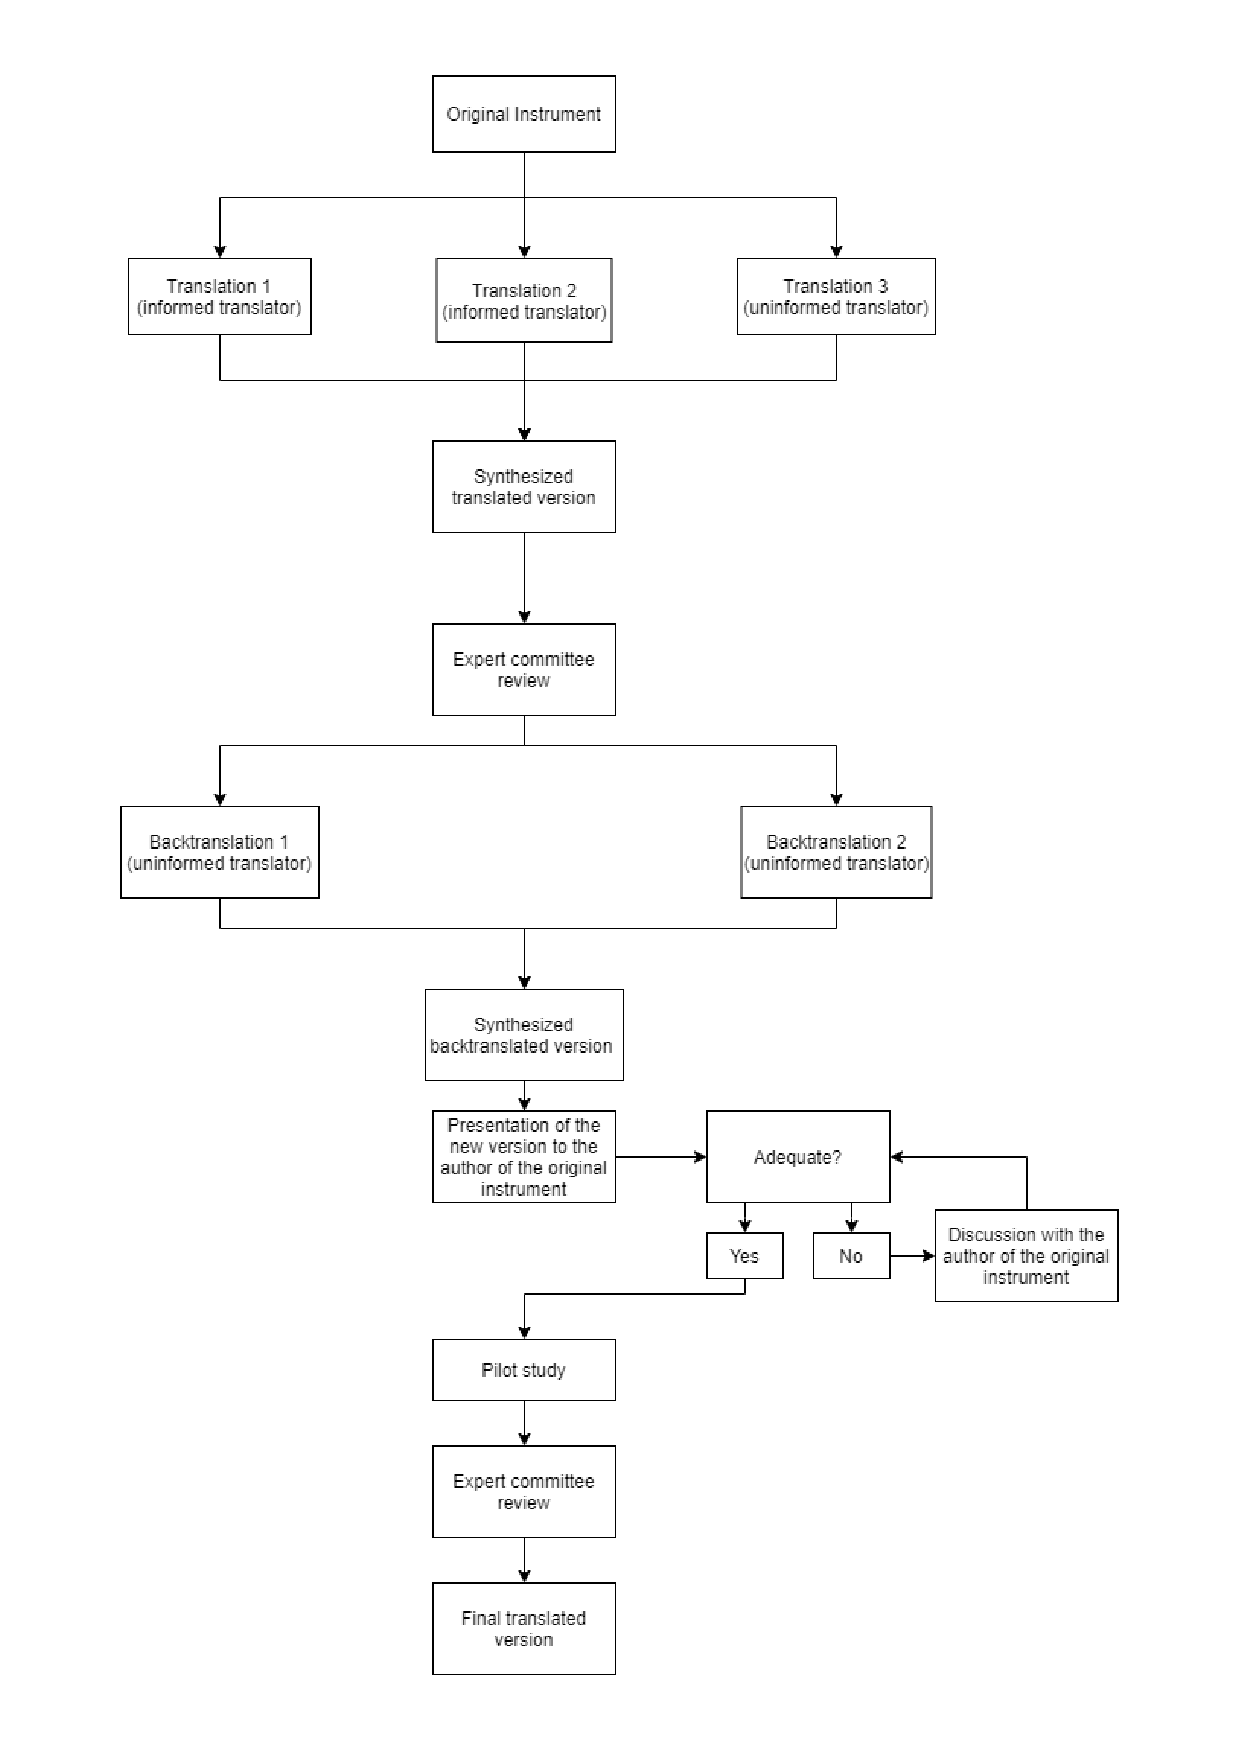
\includegraphics{cca_diagram} 

}

\caption{Stages of cross-cultural adaptation. Adapted from “Cross-Cultural Adaptation and Validation of Psychological Instruments: Some Considerations”, by J. C. Borsa, B. F. Damásio and D. R. Bandeira, 2012, Paidéia, 22(53), 423-432; “Guidelines for the Process of Cross-Cultural Adaptation of Self-Report Measures”, by D. E. Beaton, C. Bombardier, F. Guillemin and M. B. Ferraz, 2000, SPINE, 25(24), 3186-3191.}\label{fig:flowcca}
\end{figure}

\hypertarget{aditional-measures}{%
\subsection{Aditional measures}\label{aditional-measures}}

\begin{enumerate}
\def\labelenumi{\arabic{enumi}.}
\item
  \emph{Insomnia Severity Index (ISI)} (\protect\hyperlink{ref-bastien2001}{Bastien et al., 2001}; \protect\hyperlink{ref-morin2011a}{Morin et al., 2011}) is a 7-item questionnaire to assess insomnia severity and its impact on the patient's life. Raters use a 5-point scale ranging from 0 (no problem) to 4 (very severe problem). We used the Brazilian-Portuguese version (\protect\hyperlink{ref-castro}{Castro, 2011}).
\item
  \emph{The Hospital Anxiety and Depression Scale (HADS)} (\protect\hyperlink{ref-zigmond1983hospital}{Zigmond \& Snaith, 1983}) is a scale used to assess psychological distress in non-psychiatric patients. It is formed by a two-factor structure with seven items assessing Anxiety plus seven other items measuring Depression. A Brazilian-Portuguese version produced by Botega et al. (\protect\hyperlink{ref-botega1995transtornos}{1995}) was used.
\item
  \emph{Acceptance and Action Questionnaire-II (AAQ-II)} (\protect\hyperlink{ref-bond2011preliminary}{Bond et al., 2011}; \protect\hyperlink{ref-hayes2004measuring}{Hayes, Strosahl, et al., 2004}) is a measure of psychological flexibility composed by seven items rated in a scale from 1 (never true) to 7 (always true). it is scored by adding up scores for each question. Higher scoring indicate less flexibility. The Brazilian-portuguese version used in this study was produced by Barbosa and Murta (\protect\hyperlink{ref-barbosa2015propriedades}{2015}).
\end{enumerate}

\hypertarget{analytical-plan}{%
\subsection{Analytical Plan}\label{analytical-plan}}

\hypertarget{descriptive-statistics}{%
\subsubsection{Descriptive statistics}\label{descriptive-statistics}}

This phase comprise examination of response frequency and item statistics in order to assess item variation, distribution and data entry quality. Items with insufficient variation might be bad for differentiating respondents and may need to be excluded or merged into fewer categories (\protect\hyperlink{ref-dima2018}{Dima, 2018}). We'll also diagnose inter-item correlations and scan for multivariate outliers (via Mahalanobis distance) to identify if there are any anomalous response patterns.

\hypertarget{examination-of-item-properties-with-irt}{%
\subsubsection{Examination of item properties with IRT}\label{examination-of-item-properties-with-irt}}

Next, we examine item response patterns using Mokken Scaling Analysis (MSA), a non-parametric Item Response Theory (IRT) thecnique. Explain what MSA is about.

\hypertarget{scale-structure-via-factor-analysis}{%
\subsubsection{Scale structure via factor analysis}\label{scale-structure-via-factor-analysis}}

\hypertarget{reliability-estimates}{%
\subsubsection{Reliability estimates}\label{reliability-estimates}}

\hypertarget{calculation-of-global-scores}{%
\subsubsection{Calculation of global scores}\label{calculation-of-global-scores}}

\newpage

\hypertarget{partial-results}{%
\section{Partial results}\label{partial-results}}

\hypertarget{cross-cultural-adaptation}{%
\subsection{Cross-cultural adaptation}\label{cross-cultural-adaptation}}

The initial translation of SPAQ and DBAS-16 instructions, rating scale, and items was a mix of translations produced by the three (for each instrument) forward translators. To some items a determined translation was taken with minor or no modifications. Others were a merge of two or more versions with additions were it deemed necessary. The instruments versions produced in each stage of the cross-cultural adaptation process, as well as a detailed documentation of criteria for decisions, are available at \url{https://osf.io/av45j/}.

Once each stage of the translation process was completed, both instruments were submitted to appreciation by a sample of 15 subjects of the target population. Overall, participants had a good comprehension of the test items and instructions and only a single term of the DBAS-16 required alteration for a more natural reading in the target language. The final version of both DBAS-16 and SPAQ are on Appendices \ref{cads-16} and \ref{qaps}, respectively. Colocar mudança nas instruções do SPAQ.

\hypertarget{sample-description}{%
\subsection{Sample description}\label{sample-description}}

After excluding individuals who did not meet the inclusion criteria and those who failed to complete at least the first questionnaire on the survey (DBAS-16), the final sample was comprised of 1397 individuals, of which 1130 were female and 1062 reported insomnia symptoms. Sample mean age was 38.41 years (SD = 9.79, range: 18--59.80 years). There were 619 participants who reported having a formal job, and 1085 had a university degree. A detailed description of the sample is found on Table \ref{tab:tab1}.

\begin{table}

\caption{\label{tab:tab1}Sample description}
\centering
\begin{tabu} to \linewidth {>{\raggedright}X>{\centering}X}
\toprule
  & *n* = 1397\\
\midrule
Sex Male (\%) & 267 (19.1)\\
Age (mean (SD)) & 38.41 (9.79)\\
Race (\%) & \\
\hspace{1em}Asian & 48 ( 3.4)\\
\hspace{1em}Black & 331 (23.7)\\
\addlinespace
\hspace{1em}Other/Not informed & 13 ( 0.9)\\
\hspace{1em}White & 1005 (71.9)\\
Marital Status (mean (SD)) & 2.37 (1.23)\\
Educational Level (\%) & \\
\hspace{1em}Primary School & 17 ( 1.2)\\
\addlinespace
\hspace{1em}Secondary School & 295 (21.1)\\
\hspace{1em}University degree or higher & 1085 (77.7)\\
Monthly income (mean (SD)) & 9197.40 (7946.13)\\
Occupation (\%) & \\
\hspace{1em}Informal work & 46 ( 3.3)\\
\addlinespace
\hspace{1em}Regular job & 619 (44.3)\\
\hspace{1em}Retired & 29 ( 2.1)\\
\hspace{1em}Self-employed & 410 (29.3)\\
\hspace{1em}Student & 172 (12.3)\\
\hspace{1em}Unemployed & 121 ( 8.7)\\
\addlinespace
Insomnia (\%) & 1062 (76.0)\\
Region (\%) & \\
\hspace{1em}Central-West & 54 ( 3.9)\\
\hspace{1em}Northeast & 105 ( 7.6)\\
\hspace{1em}Northern & 36 ( 2.6)\\
\addlinespace
\hspace{1em}Southeast & 1083 (77.9)\\
\hspace{1em}Southern & 112 ( 8.1)\\
\bottomrule
\end{tabu}
\end{table}

\newpage

\hypertarget{next-steps}{%
\section{Next steps}\label{next-steps}}

\hypertarget{timeline}{%
\subsection{Timeline}\label{timeline}}

\begin{table}[h]
\begin{center}
\begin{threeparttable}
\caption{\label{tab:timeline_table}Timeline of events}
\begin{tabular}{cccc}
\toprule
Period & \multicolumn{1}{c}{Activities}\\
\midrule
09-10 & Do something\\
11-12 & do something else\\
\bottomrule
\end{tabular}
\end{threeparttable}
\end{center}
\end{table}

\newpage

\hypertarget{references}{%
\section{References}\label{references}}

\setlength{\parindent}{-0.5in}
\setlength{\leftskip}{0.5in}

\hypertarget{refs}{}
\begin{CSLReferences}{1}{0}
\leavevmode\vadjust pre{\hypertarget{ref-akram2020}{}}%
Akram, U., Gardani, M., Riemann, D., Akram, A., Allen, S. F., Lazuras, L., \& Johann, A. F. (2020). Dysfunctional sleep-related cognition and anxiety mediate the relationship between multidimensional perfectionism and insomnia symptoms. \emph{Cognitive Processing}, \emph{21}(1), 141--148. \url{https://doi.org/10.1007/s10339-019-00937-8}

\leavevmode\vadjust pre{\hypertarget{ref-arafat2016}{}}%
Arafat, S., Chowdhury, H., Qusar, M., \& Hafez, M. (2016). Cross {Cultural Adaptation} and {Psychometric Validation} of {Research Instruments}: A {Methodological Review}. \emph{Journal of Behavioral Health}, \emph{5}(3), 129. \url{https://doi.org/10.5455/jbh.20160615121755}

\leavevmode\vadjust pre{\hypertarget{ref-americanpsychiatricassociation2013}{}}%
Association, A. P. (Ed.). (2013). \emph{Diagnostic and statistical manual of mental disorders: {DSM}-5} (5th ed). {American Psychiatric Association}.

\leavevmode\vadjust pre{\hypertarget{ref-barbosa2015propriedades}{}}%
Barbosa, L. M., \& Murta, S. G. (2015). Propriedades psicométricas iniciais do acceptance and action questionnaire-II-versão brasileira. \emph{Psico-USF}, \emph{20}, 75--85.

\leavevmode\vadjust pre{\hypertarget{ref-bastien2001}{}}%
Bastien, C. H., Vallières, A., \& Morin, C. M. (2001). Validation of the {Insomnia Severity Index} as an outcome measure for insomnia research. \emph{Sleep Medicine}, \emph{2}(4), 297--307. \url{https://doi.org/10.1016/s1389-9457(00)00065-4}

\leavevmode\vadjust pre{\hypertarget{ref-beaton2000}{}}%
Beaton, D. E., Bombardier, C., Guillemin, F., \& Ferraz, M. B. (2000). Guidelines for the {Process} of {Cross-Cultural Adaptation} of {Self-Report Measures}: \emph{Spine}, \emph{25}(24), 3186--3191. \url{https://doi.org/10.1097/00007632-200012150-00014}

\leavevmode\vadjust pre{\hypertarget{ref-beck1979cognitive}{}}%
Beck, A. T. (1979). \emph{Cognitive therapy of depression}. Guilford press.

\leavevmode\vadjust pre{\hypertarget{ref-belanger2006}{}}%
Belanger, L., Savard, J., \& Morin, C. M. (2006). Clinical management of insomnia using cognitive therapy. \emph{Behavioral Sleep Medicine}, \emph{4}(3), 179--198. \url{https://doi.org/10.1207/s15402010bsm0403_4}

\leavevmode\vadjust pre{\hypertarget{ref-blanken2020}{}}%
Blanken, T. F., Borsboom, D., Penninx, B. W., \& Van Someren, E. J. (2020). Network outcome analysis identifies difficulty initiating sleep as a primary target for prevention of depression: A 6-year prospective study. \emph{Sleep}, \emph{43}(5), zsz288. \url{https://doi.org/gghm2s}

\leavevmode\vadjust pre{\hypertarget{ref-bond2011preliminary}{}}%
Bond, F. W., Hayes, S. C., Baer, R. A., Carpenter, K. M., Guenole, N., Orcutt, H. K., Waltz, T., \& Zettle, R. D. (2011). Preliminary psychometric properties of the acceptance and action questionnaire--II: A revised measure of psychological inflexibility and experiential avoidance. \emph{Behavior Therapy}, \emph{42}(4), 676--688.

\leavevmode\vadjust pre{\hypertarget{ref-borsaAdaptacaoValidacaoInstrumentos2012}{}}%
Borsa, J. C., Damásio, B. F., \& Bandeira, D. R. (2012). {Adaptação e validação de instrumentos psicológicos entre culturas: algumas considerações}. \emph{Paidéia (Ribeirão Preto)}, \emph{22}(53), 423--432. \url{https://doi.org/10.1590/S0103-863X2012000300014}

\leavevmode\vadjust pre{\hypertarget{ref-botega1995transtornos}{}}%
Botega, N. J., Bio, M. R., Zomignani, M. A., Garcia Jr, C., \& Pereira, W. A. (1995). Transtornos do humor em enfermaria de clínica médica e validação de escala de medida (HAD) de ansiedade e depressão. \emph{Revista de Saude Publica}, \emph{29}, 359--363.

\leavevmode\vadjust pre{\hypertarget{ref-bothelius2015}{}}%
Bothelius, K., Jernelöv, S., Fredrikson, M., McCracken, L. M., \& Kaldo, V. (2015). Measuring {Acceptance} of {Sleep Difficulties}: {The Development} of the {Sleep Problem Acceptance Questionnaire}. \emph{Sleep}, \emph{38}(11), 1815--1822. \url{https://doi.org/10.5665/sleep.5170}

\leavevmode\vadjust pre{\hypertarget{ref-boysan2010}{}}%
Boysan, M., Merey, Z., Kalafat, T., \& Kağan, M. (2010). Validation of a brief version of the dysfunctional beliefs and attitudes about sleep scale in {Turkish} sample. \emph{Procedia - Social and Behavioral Sciences}, \emph{5}, 314--317. \url{https://doi.org/10.1016/j.sbspro.2010.07.095}

\leavevmode\vadjust pre{\hypertarget{ref-brewin1996theoretical}{}}%
Brewin, C. R. (1996). Theoretical foundations of cognitive-behavior therapy for anxiety and depression. \emph{Annual Review of Psychology}, \emph{47}(1), 33--57.

\leavevmode\vadjust pre{\hypertarget{ref-carney2006}{}}%
Carney, C. E., \& Edinger, J. D. (2006). Identifying {Critical Beliefs About Sleep} in {Primary Insomnia}. \emph{Sleep}, \emph{29}(3), 342--350. \url{https://doi.org/10.1093/sleep/29.3.342}

\leavevmode\vadjust pre{\hypertarget{ref-castro}{}}%
Castro, L. S. (2011). \emph{Adaptação e validação do {Índice} de {Gravidade} de {Insônia} ({IGI})} {[}PhD thesis{]}. Universidade Federal de São Paulo.

\leavevmode\vadjust pre{\hypertarget{ref-chen2017}{}}%
Chen, P.-J., Huang, C. L.-C., Weng, S.-F., Wu, M.-P., Ho, C.-H., Wang, J.-J., Tsai, W.-C., \& Hsu, Y.-W. (2017). Relapse insomnia increases greater risk of anxiety and depression: Evidence from a population-based 4-year cohort study. \emph{Sleep Medicine}, \emph{38}, 122--129. \url{https://doi.org/10.1016/j.sleep.2017.07.016}

\leavevmode\vadjust pre{\hypertarget{ref-chow2018}{}}%
Chow, P. I., Ingersoll, K. S., Thorndike, F. P., Lord, H. R., Gonder-Frederick, L., Morin, C. M., \& Ritterband, L. M. (2018). Cognitive mechanisms of sleep outcomes in a randomized clinical trial of internet-based cognitive behavioral therapy for insomnia. \emph{Sleep Medicine}, \emph{47}, 77--85. \url{https://doi.org/10.1016/j.sleep.2017.11.1140}

\leavevmode\vadjust pre{\hypertarget{ref-chungka-fai2016}{}}%
Chung Ka-Fai, Ho Fiona Yan-Yee, \& Yeung Wing-Fai. (2016). Psychometric {Comparison} of the {Full} and {Abbreviated Versions} of the {Dysfunctional Beliefs} and {Attitudes} about {Sleep Scale}. \emph{Journal of Clinical Sleep Medicine}, \emph{12}(06), 821--828. \url{https://doi.org/10.5664/jcsm.5878}

\leavevmode\vadjust pre{\hypertarget{ref-collins2003}{}}%
Collins, D. (2003). Pretesting survey instruments: {An} overview of cognitive methods. \emph{Quality of Life Research}, \emph{12}(3), 229--238. \url{https://doi.org/10.1023/A:1023254226592}

\leavevmode\vadjust pre{\hypertarget{ref-cronlein2014}{}}%
Crönlein, T., Wagner, S., Langguth, B., Geisler, P., Eichhammer, P., \& Wetter, T. C. (2014). Are dysfunctional attitudes and beliefs about sleep unique to primary insomnia? \emph{Sleep Medicine}, \emph{15}(12), 1463--1467. \url{https://doi.org/gn3m9k}

\leavevmode\vadjust pre{\hypertarget{ref-dalrymple2010}{}}%
Dalrymple, K. L., Fiorentino, L., Politi, M. C., \& Posner, D. (2010). Incorporating {Principles} from {Acceptance} and {Commitment Therapy} into {Cognitive-Behavioral Therapy} for {Insomnia}: {A Case Example}. \emph{Journal of Contemporary Psychotherapy}, \emph{40}(4), 209--217. \url{https://doi.org/10.1007/s10879-010-9145-1}

\leavevmode\vadjust pre{\hypertarget{ref-dhyani2013}{}}%
Dhyani, M., Rajput, R., \& Gupta, R. (2013). Hindi translation and validation of dysfunctional beliefs and attitudes about sleep ({DBAS} - 16). \emph{Industrial Psychiatry Journal}, \emph{22}(1), 80--85. \url{https://doi.org/10.4103/0972-6748.123639}

\leavevmode\vadjust pre{\hypertarget{ref-dima2018}{}}%
Dima, A. L. (2018). Scale validation in applied health research: Tutorial for a 6-step {R-based} psychometrics protocol. \emph{Health Psychology and Behavioral Medicine}, \emph{6}(1), 136--161. \url{https://doi.org/10.1080/21642850.2018.1472602}

\leavevmode\vadjust pre{\hypertarget{ref-dortasjunior2016}{}}%
Dortas Junior, S. D., Lupi, O., Dias, G. A. C., Guimarães, M. B. S., \& Valle, S. O. R. (2016). {Cross-cultural adaptation and validation of health questionnaires}. \emph{Brazilian Journal of Allergy and Immunology (BJAI)}, \emph{4}(1). \url{https://doi.org/10.5935/2318-5015.20160003}

\leavevmode\vadjust pre{\hypertarget{ref-edingerjackd.2021}{}}%
Edinger J. D., Arnedt J. Todd, Bertisch Suzanne M., Carney Colleen E., Harrington John J., Lichstein Kenneth L., Sateia Michael J., Troxel Wendy M., Zhou Eric S., Kazmi Uzma, Heald Jonathan L., \& Martin Jennifer L. (2021). Behavioral and psychological treatments for chronic insomnia disorder in adults: An {American Academy} of {Sleep Medicine} systematic review, meta-analysis, and {GRADE} assessment. \emph{Journal of Clinical Sleep Medicine}, \emph{17}(2), 263--298. \url{https://doi.org/10.5664/jcsm.8988}

\leavevmode\vadjust pre{\hypertarget{ref-eidelman2016}{}}%
Eidelman, P., Talbot, L., Ivers, H., BÃÂlanger, L., Morin, C. M., \& Harvey, A. G. (2016). Change in {Dysfunctional Beliefs About Sleep} in {Behavior Therapy}, {Cognitive Therapy}, and {Cognitive-Behavioral Therapy} for {Insomnia}. \emph{Behavior Therapy}, \emph{47}(1), 102--115. \url{https://doi.org/10.1016/j.beth.2015.10.002}

\leavevmode\vadjust pre{\hypertarget{ref-epstein2015}{}}%
Epstein, J., Santo, R. M., \& Guillemin, F. (2015). A review of guidelines for cross-cultural adaptation of questionnaires could not bring out a consensus. \emph{Journal of Clinical Epidemiology}, \emph{68}(4), 435--441. \url{https://doi.org/10.1016/j.jclinepi.2014.11.021}

\leavevmode\vadjust pre{\hypertarget{ref-espie2006}{}}%
Espie, C. A., Broomfield, N. M., MacMahon, K. M. A., Macphee, L. M., \& Taylor, L. M. (2006). The attention-intention-effort pathway in the development of psychophysiologic insomnia: A theoretical review. \emph{Sleep Medicine Reviews}, \emph{10}(4), 215--245. \url{https://doi.org/10.1016/j.smrv.2006.03.002}

\leavevmode\vadjust pre{\hypertarget{ref-flakeConstructValidationSocial2017}{}}%
Flake, J. K., Pek, J., \& Hehman, E. (2017). Construct {Validation} in {Social} and {Personality Research}: {Current Practice} and {Recommendations}. \emph{Social Psychological and Personality Science}, \emph{8}(4), 370--378. \url{https://doi.org/10.1177/1948550617693063}

\leavevmode\vadjust pre{\hypertarget{ref-fortier-brochu2012}{}}%
Fortier-Brochu, E., Beaulieu-Bonneau, S., Ivers, H., \& Morin, C. M. (2012). Insomnia and daytime cognitive performance: A meta-analysis. \emph{Sleep Medicine Reviews}, \emph{16}(1), 83--94. \url{https://doi.org/10.1016/j.smrv.2011.03.008}

\leavevmode\vadjust pre{\hypertarget{ref-geisinger1994}{}}%
Geisinger, K. F. (1994). Cross-cultural normative assessment: {Translation} and adaptation issues influencing the normative interpretation of assessment instruments. \emph{Psychological Assessment}, \emph{6}(4), 304--312. \url{https://doi.org/10.1037/1040-3590.6.4.304}

\leavevmode\vadjust pre{\hypertarget{ref-gjersing2010}{}}%
Gjersing, L., Caplehorn, J. R., \& Clausen, T. (2010). Cross-cultural adaptation of research instruments: Language, setting, time and statistical considerations. \emph{BMC Medical Research Methodology}, \emph{10}(1), 13. \url{https://doi.org/10.1186/1471-2288-10-13}

\leavevmode\vadjust pre{\hypertarget{ref-guillemin1993}{}}%
Guillemin, F., Bombardier, C., \& Beaton, D. (1993). Cross-cultural adaptation of health-related quality of life measures: {Literature} review and proposed guidelines. \emph{Journal of Clinical Epidemiology}, \emph{46}(12), 1417--1432. \url{https://doi.org/10.1016/0895-4356(93)90142-N}

\leavevmode\vadjust pre{\hypertarget{ref-harris2019redcap}{}}%
Harris, P. A., Taylor, R., Minor, B. L., Elliott, V., Fernandez, M., O'Neal, L., McLeod, L., Delacqua, G., Delacqua, F., Kirby, J., et al. (2019). The REDCap consortium: Building an international community of software platform partners. \emph{Journal of Biomedical Informatics}, \emph{95}, 103208.

\leavevmode\vadjust pre{\hypertarget{ref-harris2009research}{}}%
Harris, P. A., Taylor, R., Thielke, R., Payne, J., Gonzalez, N., \& Conde, J. G. (2009). Research electronic data capture (REDCap)---a metadata-driven methodology and workflow process for providing translational research informatics support. \emph{Journal of Biomedical Informatics}, \emph{42}(2), 377--381.

\leavevmode\vadjust pre{\hypertarget{ref-harvey2002}{}}%
Harvey, A. G. (2002). A cognitive model of insomnia. \emph{Behaviour Research and Therapy}, \emph{40}(8), 869--893. \url{https://doi.org/fwxq35}

\leavevmode\vadjust pre{\hypertarget{ref-harvey2014}{}}%
Harvey, A. G., Bélanger, L., Talbot, L., Eidelman, P., Beaulieu-Bonneau, S., Fortier-Brochu, É., Ivers, H., Lamy, M., Hein, K., Soehner, A. M., Mérette, C., \& Morin, C. M. (2014). Comparative efficacy of behavior therapy, cognitive therapy, and cognitive behavior therapy for chronic insomnia: A randomized controlled trial. \emph{Journal of Consulting and Clinical Psychology}, \emph{82}(4), 670--683. \url{https://doi.org/10.1037/a0036606}

\leavevmode\vadjust pre{\hypertarget{ref-harvey2017}{}}%
Harvey, A. G., Dong, L., Bélanger, L., \& Morin, C. M. (2017). Mediators and treatment matching in behavior therapy, cognitive therapy and cognitive behavior therapy for chronic insomnia. \emph{Journal of Consulting and Clinical Psychology}, \emph{85}(10), 975--987. \url{https://doi.org/10.1037/ccp0000244}

\leavevmode\vadjust pre{\hypertarget{ref-hayes2004mindfulness}{}}%
Hayes, S. C., Follette, V. M., \& Linehan, M. (2004). \emph{Mindfulness and acceptance: Expanding the cognitive-behavioral tradition}. Guilford Press.

\leavevmode\vadjust pre{\hypertarget{ref-hayes2011acceptance}{}}%
Hayes, S. C., Strosahl, K. D., \& Wilson, K. G. (2011). \emph{Acceptance and commitment therapy: The process and practice of mindful change}. Guilford press.

\leavevmode\vadjust pre{\hypertarget{ref-hayes2004measuring}{}}%
Hayes, S. C., Strosahl, K., Wilson, K. G., Bissett, R. T., Pistorello, J., Toarmino, D., Polusny, M. A., Dykstra, T. A., Batten, S. V., Bergan, J., et al. (2004). Measuring experiential avoidance: A preliminary test of a working model. \emph{The Psychological Record}, \emph{54}(4), 553--578.

\leavevmode\vadjust pre{\hypertarget{ref-herdmanModelEquivalenceCultural1998}{}}%
Herdman, M., Fox-Rushby, J., \& Badia, X. (1998). A model of equivalence in the cultural adaptation of {HRQoL} instruments. \emph{Quality of Life Research}, \emph{7}, 323--335.

\leavevmode\vadjust pre{\hypertarget{ref-hertenstein2014}{}}%
Hertenstein, E., Thiel, N., Lüking, M., Külz, A. K., Schramm, E., Baglioni, C., Spiegelhalder, K., Riemann, D., \& Nissen, C. (2014). Quality of {Life Improvements} after {Acceptance} and {Commitment Therapy} in {Nonresponders} to {Cognitive Behavioral Therapy} for {Primary Insomnia}. \emph{Psychotherapy and Psychosomatics}, \emph{83}(6), 371--373. \url{https://doi.org/10.1159/000365173}

\leavevmode\vadjust pre{\hypertarget{ref-jansson-frojmark2008b}{}}%
Jansson-Fröjmark, M., \& Lindblom, K. (2008). A bidirectional relationship between anxiety and depression, and insomnia? {A} prospective study in the general population. \emph{Journal of Psychosomatic Research}, \emph{64}(4), 443--449. \url{https://doi.org/10.1016/j.jpsychores.2007.10.016}

\leavevmode\vadjust pre{\hypertarget{ref-johnson2006}{}}%
Johnson, E. O., Roth, T., \& Breslau, N. (2006). The association of insomnia with anxiety disorders and depression: Exploration of the direction of risk. \emph{Journal of Psychiatric Research}, \emph{40}(8), 700--708. \url{https://doi.org/d5k6f6}

\leavevmode\vadjust pre{\hypertarget{ref-semtools}{}}%
Jorgensen, T. D., Pornprasertmanit, S., Schoemann, A. M., \& Rosseel, Y. (2021). \emph{\texttt{semTools}: {U}seful tools for structural equation modeling}. \url{https://CRAN.R-project.org/package=semTools}

\leavevmode\vadjust pre{\hypertarget{ref-koller2012}{}}%
Koller, M., Kantzer, V., Mear, I., Zarzar, K., Martin, M., Greimel, E., Bottomley, A., Arnott, M., Kuliś, D., \& The ISOQOL TCA-SIG. (2012). The process of reconciliation: Evaluation of guidelines for translating quality-of-life questionnaires. \emph{Expert Review of Pharmacoeconomics \& Outcomes Research}, \emph{12}(2), 189--197. \url{https://doi.org/10.1586/erp.11.102}

\leavevmode\vadjust pre{\hypertarget{ref-lancee2019}{}}%
Lancee, J., Effting, M., van der Zweerde, T., van Daal, L., van Straten, A., \& Kamphuis, J. H. (2019). Cognitive processes mediate the effects of insomnia treatment: Evidence from a randomized wait-list controlled trial. \emph{Sleep Medicine}, \emph{54}, 86--93. \url{https://doi.org/10.1016/j.sleep.2018.09.029}

\leavevmode\vadjust pre{\hypertarget{ref-lang2017}{}}%
Lang, C., Brand, S., Holsboer-Trachsler, E., Pühse, U., Colledge, F., \& Gerber, M. (2017). Validation of the {German} version of the short form of the dysfunctional beliefs and attitudes about sleep scale ({DBAS-16}). \emph{Neurological Sciences}, \emph{38}(6), 1047--1058. \url{https://doi.org/10.1007/s10072-017-2921-x}

\leavevmode\vadjust pre{\hypertarget{ref-li2016}{}}%
Li, L., Wu, C., Gan, Y., Qu, X., \& Lu, Z. (2016). Insomnia and the risk of depression: A meta-analysis of prospective cohort studies. \emph{BMC Psychiatry}, \emph{16}, 375. \url{https://doi.org/f9bsxr}

\leavevmode\vadjust pre{\hypertarget{ref-lundh2005}{}}%
Lundh, L.-G. (2005). The {Role} of {Acceptance} and {Mindfulness} in the {Treatment} of {Insomnia}. \emph{Journal of Cognitive Psychotherapy}, \emph{19}(1), 29--39. \url{https://doi.org/10.1891/jcop.19.1.29.66331}

\leavevmode\vadjust pre{\hypertarget{ref-lundh2000}{}}%
Lundh, L.-G., \& Broman, J.-E. (2000). Insomnia as an interaction between sleep-interfering and sleep-interpreting processes. \emph{Journal of Psychosomatic Research}, \emph{49}(5), 299--310. \url{https://doi.org/10.1016/S0022-3999(00)00150-1}

\leavevmode\vadjust pre{\hypertarget{ref-maccallum1996}{}}%
MacCallum, R. C., Browne, M. W., \& Sugawara, H. M. (1996). Power analysis and determination of sample size for covariance structure modeling. \emph{Psychological Methods}, \emph{1}(2), 130--149. \url{https://doi.org/10.1037/1082-989X.1.2.130}

\leavevmode\vadjust pre{\hypertarget{ref-marques2015}{}}%
Marques, D. R., Allen Gomes, A., Clemente, V., Santos, J. M., \& Castelo-Branco, M. (2015). Hyperarousal and failure to inhibit wakefulness in primary insomnia: "``Birds of a feather"? \emph{Sleep and Biological Rhythms}, \emph{13}(3), 219--228. \url{https://doi.org/10.1111/sbr.12115}

\leavevmode\vadjust pre{\hypertarget{ref-montserratsanchez-ortuno2010}{}}%
Montserrat Sánchez-Ortuño, M., \& Edinger, J. D. (2010). A penny for your thoughts: {Patterns} of sleep-related beliefs, insomnia symptoms and treatment outcome. \emph{Behaviour Research and Therapy}, \emph{48}(2), 125--133. \url{https://doi.org/10.1016/j.brat.2009.10.003}

\leavevmode\vadjust pre{\hypertarget{ref-morin1993insomnia}{}}%
Morin, C. M. (1993). \emph{Insomnia: Psychological assessment and management.} Guilford press.

\leavevmode\vadjust pre{\hypertarget{ref-morin2011a}{}}%
Morin, C. M., Belleville, G., Bélanger, L., \& Ivers, H. (2011). \href{https://www.ncbi.nlm.nih.gov/pmc/articles/PMC3079939}{The {Insomnia Severity Index}: {Psychometric Indicators} to {Detect Insomnia Cases} and {Evaluate Treatment Response}}. \emph{Sleep}, \emph{34}(5), 601--608.

\leavevmode\vadjust pre{\hypertarget{ref-morin1993}{}}%
Morin, C. M., Stone, J., Trinkle, D., Mercer, J., \& Remsberg, S. (1993). Dysfunctional beliefs and attitudes about sleep among older adults with and without insomnia complaints. \emph{Psychology and Aging}, \emph{8}(3), 463--467. \url{https://doi.org/frwwvp}

\leavevmode\vadjust pre{\hypertarget{ref-morin2007a}{}}%
Morin, C. M., Vallières, A., \& Ivers, H. (2007). Dysfunctional {Beliefs} and {Attitudes} about {Sleep} ({DBAS}): {Validation} of a {Brief Version} ({DBAS-16}). \emph{Sleep}, \emph{30}(11), 1547--1554. \url{https://doi.org/10.1093/sleep/30.11.1547}

\leavevmode\vadjust pre{\hypertarget{ref-neckelmann2007}{}}%
Neckelmann, D., Mykletun, A., \& Dahl, A. A. (2007). Chronic insomnia as a risk factor for developing anxiety and depression. \emph{Sleep}, \emph{30}(7), 873--880. \url{https://doi.org/gf26g2}

\leavevmode\vadjust pre{\hypertarget{ref-norell-clarke2021}{}}%
Norell-Clarke, A., Hagström, M., \& Jansson-Fröjmark, M. (2021). Sleep-{Related Cognitive Processes} and the {Incidence} of {Insomnia Over Time}: {Does Anxiety} and {Depression Impact} the {Relationship}? \emph{Frontiers in Psychology}, \emph{12}. \url{https://doi.org/gk8x3v}

\leavevmode\vadjust pre{\hypertarget{ref-ong2012}{}}%
Ong, J. C., Ulmer, C. S., \& Manber, R. (2012). Improving sleep with mindfulness and acceptance: {A} metacognitive model of insomnia. \emph{Behaviour Research and Therapy}, \emph{50}(11), 651--660. \url{https://doi.org/f4fczt}

\leavevmode\vadjust pre{\hypertarget{ref-perlis1997}{}}%
Perlis, M. L., Giles, D. E., Mendelson, W. B., Bootzin, R. R., \& Wyatt, J. K. (1997). Psychophysiological insomnia: The behavioural model and a neurocognitive perspective. \emph{Journal of Sleep Research}, \emph{6}(3), 179--188. \url{https://doi.org/fcrnvj}

\leavevmode\vadjust pre{\hypertarget{ref-R-base}{}}%
R Core Team. (2022). \emph{R: A language and environment for statistical computing}. R Foundation for Statistical Computing. \url{https://www.R-project.org/}

\leavevmode\vadjust pre{\hypertarget{ref-reichenheim2007}{}}%
Reichenheim, M. E., \& Moraes, C. L. (2007). {Operacionalização de adaptação transcultural de instrumentos de aferição usados em epidemiologia}. \emph{Revista de Saúde Pública}, \emph{41}(4), 665--673. \url{https://doi.org/10.1590/S0034-89102006005000035}

\leavevmode\vadjust pre{\hypertarget{ref-sadler2013}{}}%
Sadler, P., McLaren, S., \& Jenkins, M. (2013). A psychological pathway from insomnia to depression among older adults. \emph{International Psychogeriatrics}, \emph{25}(8), 1375--1383. \url{https://doi.org/10.1017/S1041610213000616}

\leavevmode\vadjust pre{\hypertarget{ref-taylor2005}{}}%
Taylor, D. J., Lichstein, K. L., Durrence, H. H., Reidel, B. W., \& Bush, A. J. (2005). Epidemiology of {Insomnia}, {Depression}, and {Anxiety}. \emph{Sleep}, \emph{28}(11), 1457--1464. \url{https://doi.org/gg5k3t}

\leavevmode\vadjust pre{\hypertarget{ref-thakral2020}{}}%
Thakral, M., Von Korff, M., McCurry, S. M., Morin, C. M., \& Vitiello, M. V. (2020). Changes in dysfunctional beliefs about sleep after cognitive behavioral therapy for insomnia: {A} systematic literature review and meta-analysis. \emph{Sleep Medicine Reviews}, \emph{49}, 101230. \url{https://doi.org/10.1016/j.smrv.2019.101230}

\leavevmode\vadjust pre{\hypertarget{ref-vanwidenfelt2005}{}}%
van Widenfelt, B. M., Treffers, P. D. A., de Beurs, E., Siebelink, B. M., \& Koudijs, E. (2005). Translation and {Cross-Cultural Adaptation} of {Assessment Instruments Used} in {Psychological Research With Children} and {Families}. \emph{Clinical Child and Family Psychology Review}, \emph{8}(2), 135--147. \url{https://doi.org/10.1007/s10567-005-4752-1}

\leavevmode\vadjust pre{\hypertarget{ref-wild2005}{}}%
Wild, D., Grove, A., Martin, M., Eremenco, S., McElroy, S., Verjee-Lorenz, A., \& Erikson, P. (2005). Principles of {Good Practice} for the {Translation} and {Cultural Adaptation Process} for {Patient-Reported Outcomes} ({PRO}) {Measures}: {Report} of the {ISPOR Task Force} for {Translation} and {Cultural Adaptation}. \emph{Value in Health}, \emph{8}(2), 94--104. \url{https://doi.org/10.1111/j.1524-4733.2005.04054.x}

\leavevmode\vadjust pre{\hypertarget{ref-zigmond1983hospital}{}}%
Zigmond, A. S., \& Snaith, R. P. (1983). The hospital anxiety and depression scale. \emph{Acta Psychiatrica Scandinavica}, \emph{67}(6), 361--370.

\end{CSLReferences}


\clearpage

\begin{appendix}
\section{Crenças e Atitudes Disfuncionais sobre o Sono (CADS-16)}
\label{cads-16}

Uma série de afirmações refletindo as crenças e atitudes das pessoas em relação ao sono estão listadas abaixo. Por favor, indique o quanto você concorda ou discorda de cada afirmação. Não há respostas certas ou erradas. Para cada afirmação, circule o número que corresponde à sua \underline{crença pessoal}. Por favor, responda todos as afirmações, mesmo que não se apliquem diretamente à sua situação.
\smallskip

\begin{flushleft}

{\setstretch{1.0}
\begin{center}
Discordo \hfill Concordo\\
Fortemente \hfill Fortemente
\end{center}

\medskip
\hrule
\medskip

\hspace*{6mm}\makebox[\linewidth][s]{0 1 2 3 4 5 6 \textcircled{7} 8 9 10 } \par

\bigskip
1. Preciso de 8 horas de sono para me sentir revigorado(a) e funcionar bem durante o dia.
\medskip
\hrule
\medskip
\hspace*{6mm}\makebox[\linewidth][s]{0 1 2 3 4 5 6 7 8 9 10 } \par


\bigskip
2. Quando não durmo o suficiente à noite, preciso recuperar o sono no dia seguinte com um cochilo ou dormindo mais na próxima noite.
\medskip
\hrule
\medskip
\hspace*{6mm}\makebox[\linewidth][s]{0 1 2 3 4 5 6 7 8 9 10 } \par

\bigskip
3. Estou preocupado(a) que a insônia crônica possa trazer consequências graves em minha saúde física. 
\medskip
\hrule
\medskip
\hspace*{6mm}\makebox[\linewidth][s]{0 1 2 3 4 5 6 7 8 9 10 } \par

\bigskip
4. Estou preocupado(a) que eu talvez perca o controle sobre minha habilidade de dormir.
\medskip
\hrule
\medskip
\hspace*{6mm}\makebox[\linewidth][s]{0 1 2 3 4 5 6 7 8 9 10 } \par

\bigskip
5. Sei que uma noite de sono ruim vai interferir nas minhas atividades cotidianas no dia seguinte.
\medskip
\hrule
\medskip
\hspace*{6mm}\makebox[\linewidth][s]{0 1 2 3 4 5 6 7 8 9 10 } \par

\bigskip
6. Para estar alerta e funcionar bem durante o dia, eu acredito que seria melhor tomar um remédio para dormir do que ter uma noite de sono ruim.
\medskip
\hrule
\medskip
\hspace*{6mm}\makebox[\linewidth][s]{0 1 2 3 4 5 6 7 8 9 10 } \par

\bigskip
7. Quando me sinto irritado(a), deprimido(a), ou ansioso(a) durante o dia, provavelmente foi porque não dormi bem na noite anterior. 
\medskip
\hrule
\medskip
\hspace*{6mm}\makebox[\linewidth][s]{0 1 2 3 4 5 6 7 8 9 10 } \par

\bigskip
8. Quando durmo mal uma noite, sei que irá atrapalhar meu sono pelo resto da semana. 
\medskip
\hrule
\medskip
\hspace*{6mm}\makebox[\linewidth][s]{0 1 2 3 4 5 6 7 8 9 10 } \par

\bigskip
9.	Sem uma noite de sono adequada, eu mal consigo funcionar no dia seguinte. 
\medskip
\hrule
\medskip
\hspace*{6mm}\makebox[\linewidth][s]{0 1 2 3 4 5 6 7 8 9 10 } \par

\bigskip
10.	Não consigo prever se vou ter uma noite de sono boa ou ruim. 
\medskip
\hrule
\medskip
\hspace*{6mm}\makebox[\linewidth][s]{0 1 2 3 4 5 6 7 8 9 10 } \par

\bigskip
11.	Tenho pouco controle sobre as consequências negativas de um sono ruim. 
\medskip
\hrule
\medskip
\hspace*{6mm}\makebox[\linewidth][s]{0 1 2 3 4 5 6 7 8 9 10 } \par

\bigskip
12.	Quando me sinto cansado(a), sem energia, ou não funciono bem durante o dia, geralmente é porque não dormi bem na noite anterior. 
\medskip
\hrule
\medskip
\hspace*{6mm}\makebox[\linewidth][s]{0 1 2 3 4 5 6 7 8 9 10 } \par

\bigskip
13.	Acredito que a insônia seja essencialmente o resultado de um desequilíbrio do meu organismo. 
\medskip
\hrule
\medskip
\hspace*{6mm}\makebox[\linewidth][s]{0 1 2 3 4 5 6 7 8 9 10 } \par

\bigskip
14.	Sinto que a insônia está arruinando minha capacidade de aproveitar a vida e me impede de fazer o que eu quero. 
\medskip
\hrule
\medskip
\hspace*{6mm}\makebox[\linewidth][s]{0 1 2 3 4 5 6 7 8 9 10 } \par

\bigskip
15.	Medicação é provavelmente a única solução para a minha falta de sono.  
\medskip
\hrule
\medskip
\hspace*{6mm}\makebox[\linewidth][s]{0 1 2 3 4 5 6 7 8 9 10 } \par

\bigskip
16.	Evito ou cancelo compromissos (sociais, familiares) após uma noite de sono ruim.
\medskip
\hrule
\medskip
\hspace*{6mm}\makebox[\linewidth][s]{0 1 2 3 4 5 6 7 8 9 10 } \par
}

\end{flushleft}

\section{Questionário de Aceitação dos Problemas no Sono (QAPS)}
\label{qaps}

Abaixo você irá encontrar uma lista de afirmações. Por favor, avalie o quanto você concorda com cada frase escolhendo uma alternativa. Responda da melhor forma que puder mesmo que você não tenha (mais) problemas de sono, ou que eles sejam pouco frequentes. Poucas pessoas tem um sono perfeito todas as noites. Deste modo, pense em qualquer dificuldade com sono que tenha, ou já tenha tido, por menor que seja, e responda de acordo.

\begin{table}[h]
\begin{tabular}{ccccccc}
0 & 1 & 2 & 3 & 4 & 5 & 6 \\
Discordo & Concordo & Concordo & Concordo & Concordo & Concordo & Concordo \\
 & muito & levemente & parcialmente & moderadamente & quase & completamente \\
 & pouco &  &  &  & completamente & 
\end{tabular}
\end{table}

\begin{table}[h]
\centering
\begin{tabular}{lllllllll}
1. & Embora as coisas tenham mudado,           & 0 & 1 & 2 & 3 & 4 & 5 & 6 \\
   & estou vivendo uma vida normal             &   &   &   &   &   &   &   \\
   & apesar dos meus problemas de sono.        &   &   &   &   &   &   &   \\
   &                                           &   &   &   &   &   &   &   \\
2. & Eu levo uma vida plena                    & 0 & 1 & 2 & 3 & 4 & 5 & 6 \\
   & apesar de ter problemas de sono.          &   &   &   &   &   &   &   \\
   &                                           &   &   &   &   &   &   &   \\
3. & Minha vida está indo bem                  & 0 & 1 & 2 & 3 & 4 & 5 & 6 \\
   & apesar dos meus problemas de sono         &   &   &   &   &   &   &   \\
   &                                           &   &   &   &   &   &   &   \\
4. & Apesar dos problemas de sono, agora estou & 0 & 1 & 2 & 3 & 4 & 5 & 6 \\
   & seguindo um certo curso na minha vida.    &   &   &   &   &   &   &   \\
   &                                           &   &   &   &   &   &   &   \\
5. & Manter meus problemas de sono sob         & 0 & 1 & 2 & 3 & 4 & 5 & 6 \\
   & controle é minha maior prioridade.        &   &   &   &   &   &   &   \\
   &                                           &   &   &   &   &   &   &   \\
6. & Eu preciso me concentrar em me livrar dos & 0 & 1 & 2 & 3 & 4 & 5 & 6 \\
   & meus problemas de sono.                   &   &   &   &   &   &   &   \\
   &                                           &   &   &   &   &   &   &   \\
7. & É importante eu continuar lutando contra  & 0 & 1 & 2 & 3 & 4 & 5 & 6 \\
   & meus problemas de sono.                   &   &   &   &   &   &   &   \\
   &                                           &   &   &   &   &   &   &   \\
8. & Meus pensamentos e sentimentos sobre      & 0 & 1 & 2 & 3 & 4 & 5 & 6 \\
   & meus problemas de sono devem mudar        &   &   &   &   &   &   &   \\
   & antes de eu dar passos importantes na     &   &   &   &   &   &   &   \\
   & minha vida.                               &   &   &   &   &   &   &  
\end{tabular}
\end{table}

\section{Reconciliation: decisions and documentation form}
\label{appendix:form}
Adapted from: Koller, M., Kantzer, V., Mear, I., Zarzar, K., Martin, M., Greimel, E., ... \& ISOQOL TCA-SIG. (2012). The process of reconciliation: evaluation of guidelines for translating quality-of-life questionnaires. \textit{Expert review of pharmacoeconomics \& outcomes research, 12}(2), 189-197.
\begin{flushleft}
\subsection{Parte I: decisões}

\subsection{Opções de decisões para a tradução reconciliada}
1.	Tradução A como está\\
2.	Tradução B como está\\
3.	Tradução C como está\\
4.	A com pequenas modificações\\
5.	B com pequenas modificações\\
6.	C com pequenas modificações\\
7.	Mesclar A, B e C como elas são, com A adaptado de B e C\\
8.	Mesclar A, B e C como elas são, com B adaptado de A e B\\
9.	Mesclar A, B e C como elas são, com C adaptado de A e B\\
10.	Mesclar A e B como elas são, com B adaptado de A\\
11.	Mesclar A e B como elas são, com A adaptado de B\\
12.	Mesclar A e C como elas são, com C adaptado de A\\
13.	Mesclar A e C como elas são, com A adaptado de C\\
14.	Mesclar B e C como elas são, com B adaptado de C\\
15.	Mesclar B e C como elas são, com C adaptado de B\\
16.	Mesclar A e B com modificações/adições, com A adaptado de B\\
17.	Mesclar A e B com modificações/adições, com B adaptado de A\\
18.	Preparar uma tradução completamente nova C\\

\subsection{Critérios de decisão para escolher qualquer uma das opções acima}

\textbf{1.	Fonte e compreensibilidade}

1.1.	 Reflete melhor as definições conceituais e o significado do texto de origem\\
1.2.	 Reflete melhor a ênfase do texto de origem (i.e., qual é o ponto principal do texto de origem)\\
1.3.	 É compreensível para um leigo sem conhecimentos médicos\\
1.4.	 É compreensível para uma população de diversos níveis educacionais\\
1.5.	 É o mais próximo possível do texto de origem\\
1.6.	 É lido com mais naturalidade no idioma de destino\\
\textbf{2.	Cultural}\\
2.1.	 É culturalmente apropriado no âmbito de tópicos sensíveis\\
2.2.	 É culturalmente apropriado no âmbito das diferenças culturais da vida\\
\textbf{3.	Gramatical}\\
3.1.	 A sintaxe está correta\\
3.2.	 As formas e tempos verbais estão corretos\\
3.3.	 Gênero e número estão adaptados e corretos\\
3.4.	 Outros elementos estão corretos (especialmente artigos e preposições)\\
\textbf{4.	Terminologia}\\
4.1.	 Inclui todas as palavras-chave\\
4.2.	 É semanticamente preciso\\
4.3.	 O vocabulário/terminologia é consistente em toda a tradução\\

\subsection{Parte II: Documentação do processo de reconciliação}

Tradução A:\\
Tradução B:\\
Tradução C:\\
Tradução reconciliada:\\
Opção de decisão: escolher uma das opções 1 a 18\\
Critérios de decisão: escolher dentre os critérios 1.1 a 4.3
\end{flushleft}
\end{appendix}

\end{document}
